\subsection{Derivative Computation} \label{sec:derivatives}

Computation of derivative-based quantities is important in data analysis. Examples include vorticity
(curl) computation from velocity fields to identify vortical structures, gradient computation for
accurate Morse segmentation and shading, and ridge extraction (e.g. for Lagrangian coherent
structures). In this paper, derivatives are always computed using finite differences, which is
common in practice. Here we use 32 bits for quantization in this section to ensure enough precision for
finite differences. We always compute finite differences on the finest resolution grid to avoid
computing distances between quantities defined on grids of different resolutions.

\begin{figure*}[h]
\centering
\subcaptionbox{\emph{boiler}}
{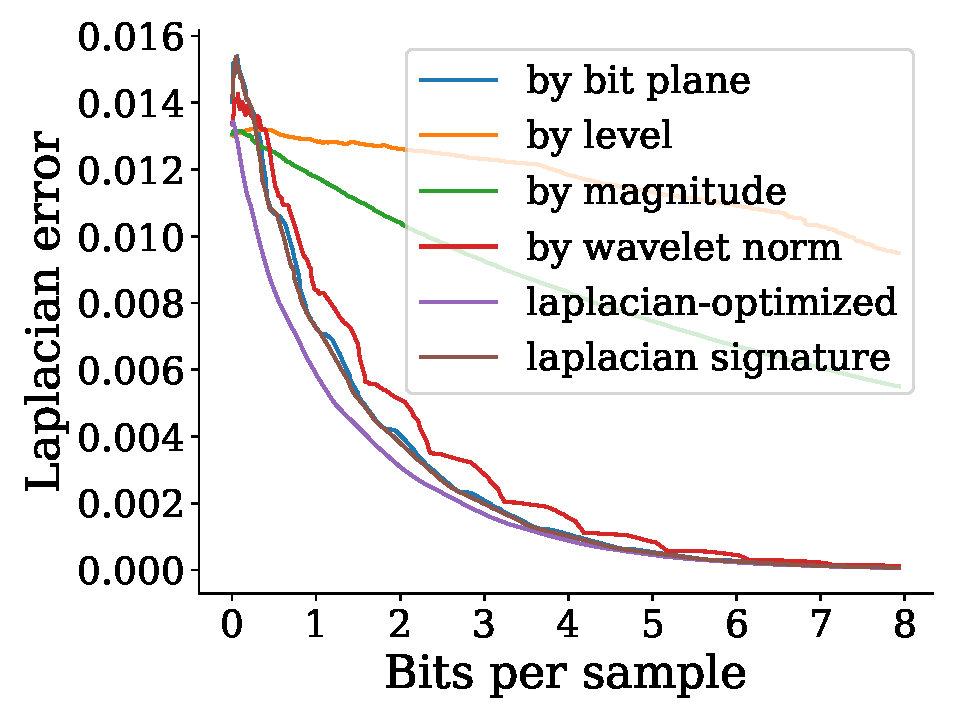
\includegraphics[width=0.24\linewidth]{laplacian/laplacian-optimized-boiler}}
\subcaptionbox{\emph{diffusivity}}
{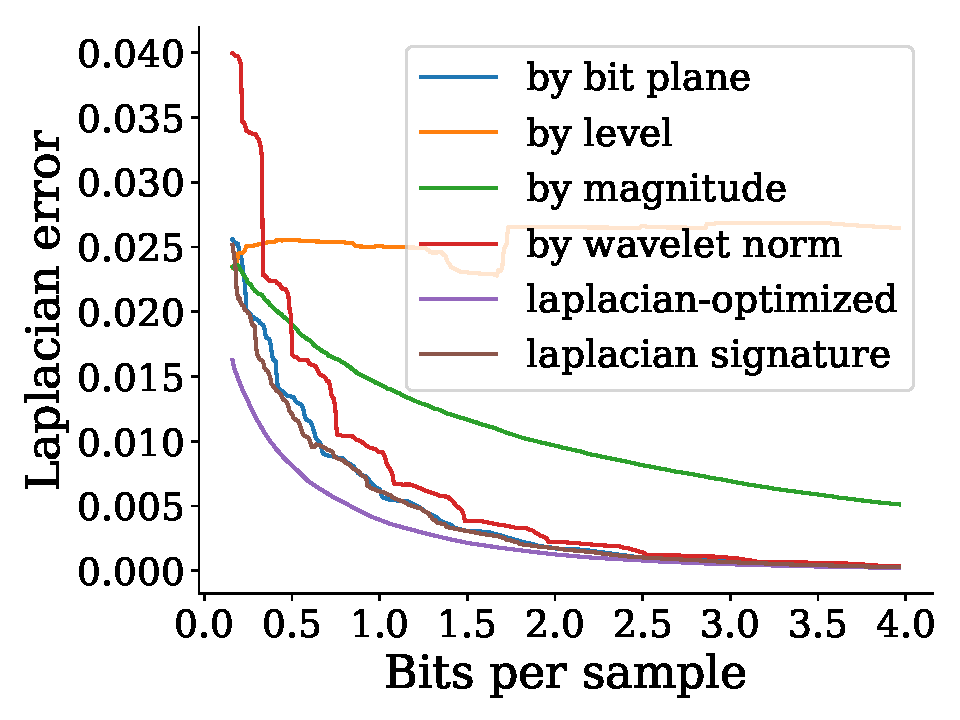
\includegraphics[width=0.24\linewidth]{laplacian/laplacian-optimized-diffusivity}}
\subcaptionbox{\emph{turbulence}}
{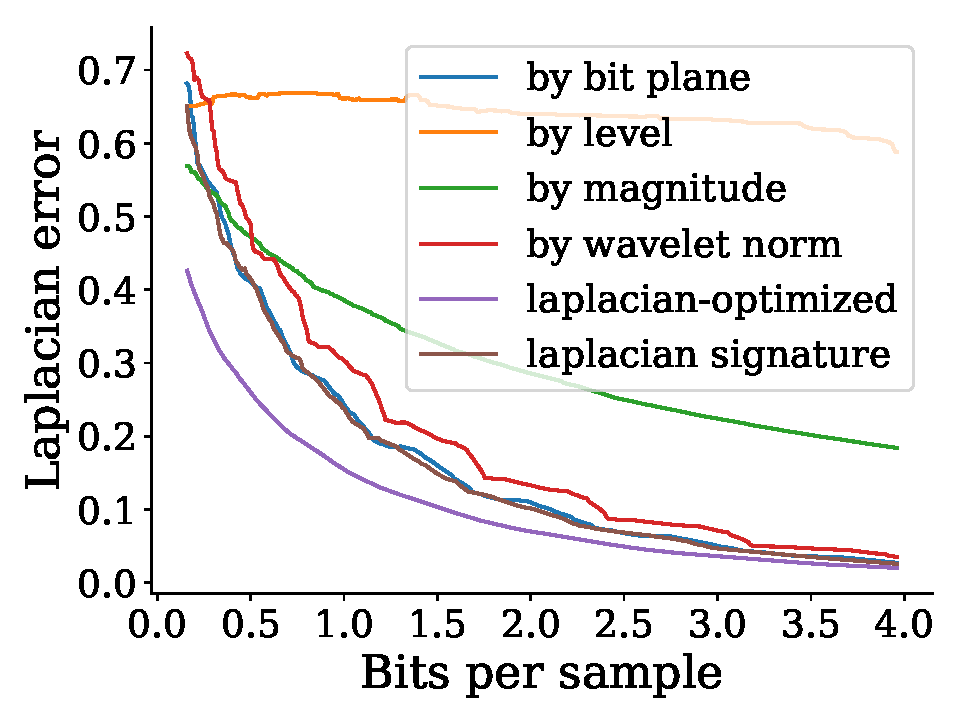
\includegraphics[width=0.24\linewidth]{laplacian/laplacian-optimized-turbulence}}
\subcaptionbox{\emph{pressure}}
{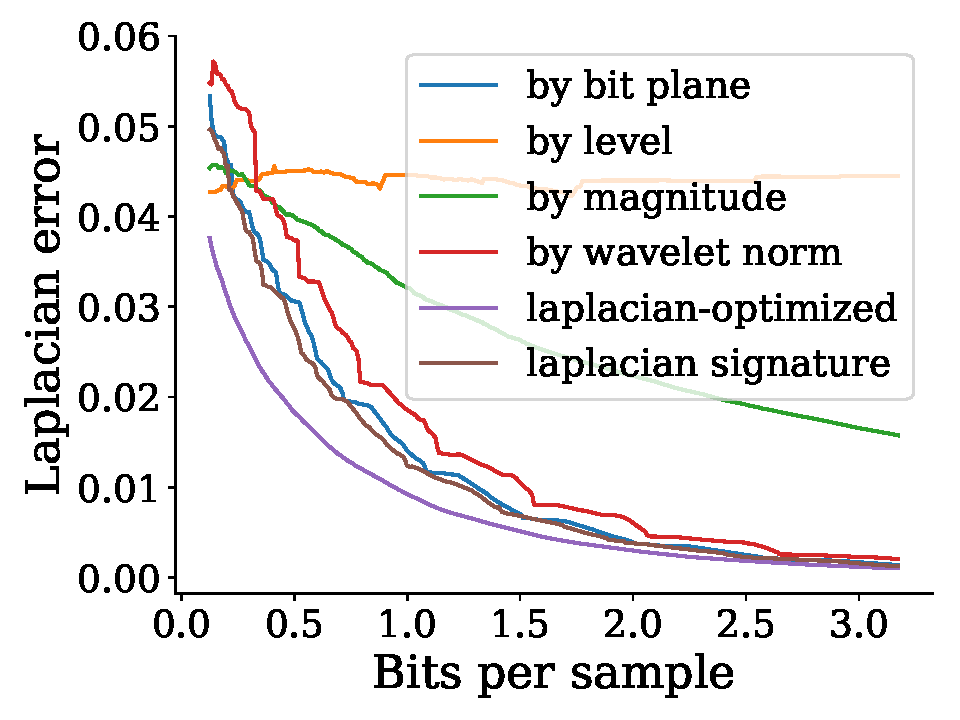
\includegraphics[width=0.24\linewidth]{laplacian/laplacian-optimized-pressure}}
\caption{Laplacian error comparison among streams. The plots are truncated to better highlight
differences without discarding important information. In all cases, in terms of error, $\slop <
\slsg < \sbit < \swav < \smag < \slvl$.}
\label{fig:laplacian-error-comparison}
\end{figure*}

\begin{figure*}[t]
        \centering
        \subcaptionbox{\emph{boiler}}
        {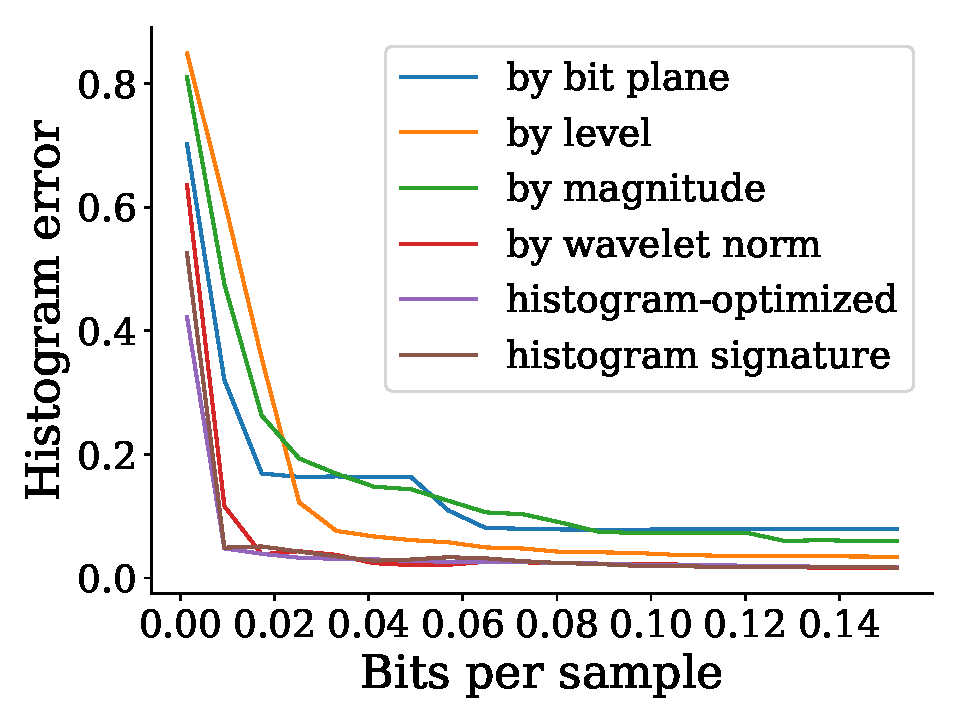
\includegraphics[width=0.24\linewidth]{histogram/histogram-optimized-boiler}}
        \subcaptionbox{\emph{diffusivity}}
        {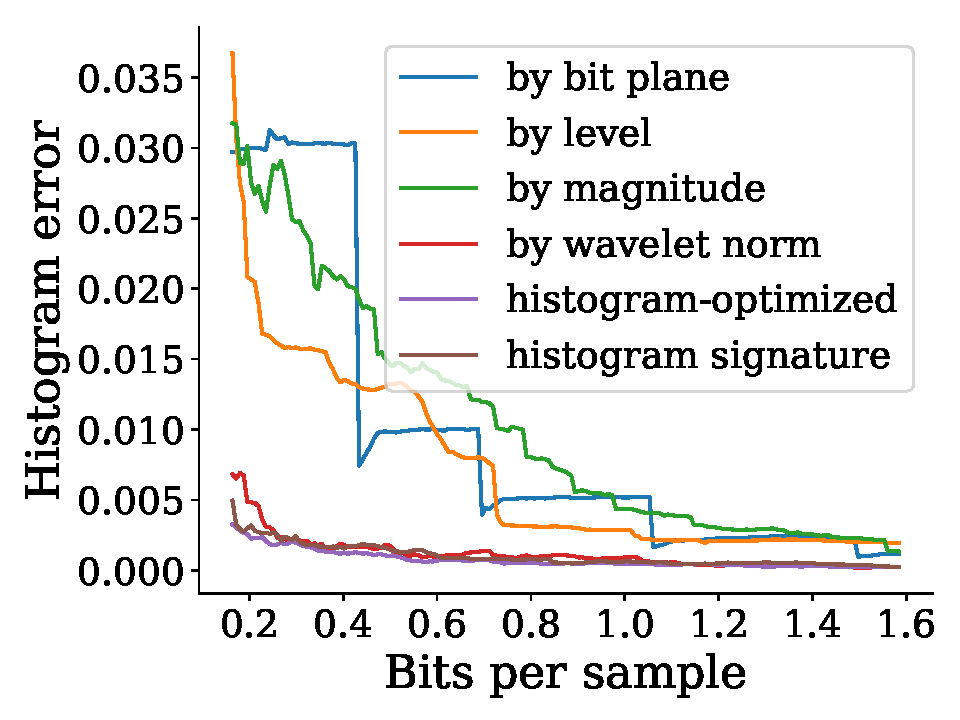
\includegraphics[width=0.24\linewidth]{histogram/histogram-optimized-diffusivity}}
        \subcaptionbox{\emph{kingsnake}}
        {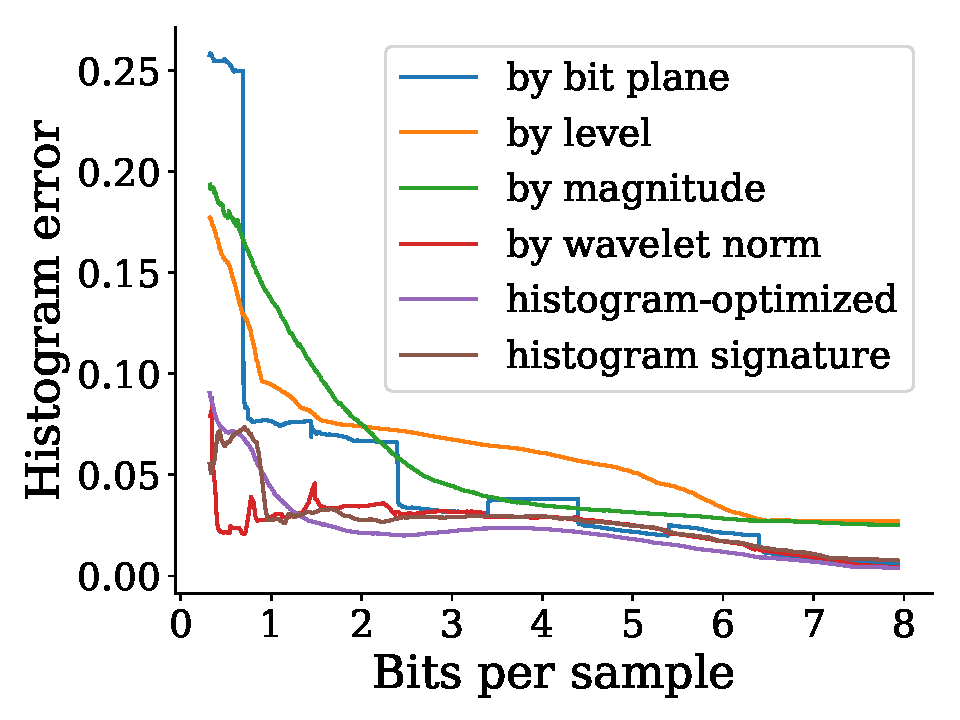
\includegraphics[width=0.24\linewidth]{histogram/histogram-optimized-kingsnake}}
        \subcaptionbox{\emph{foam}}
        {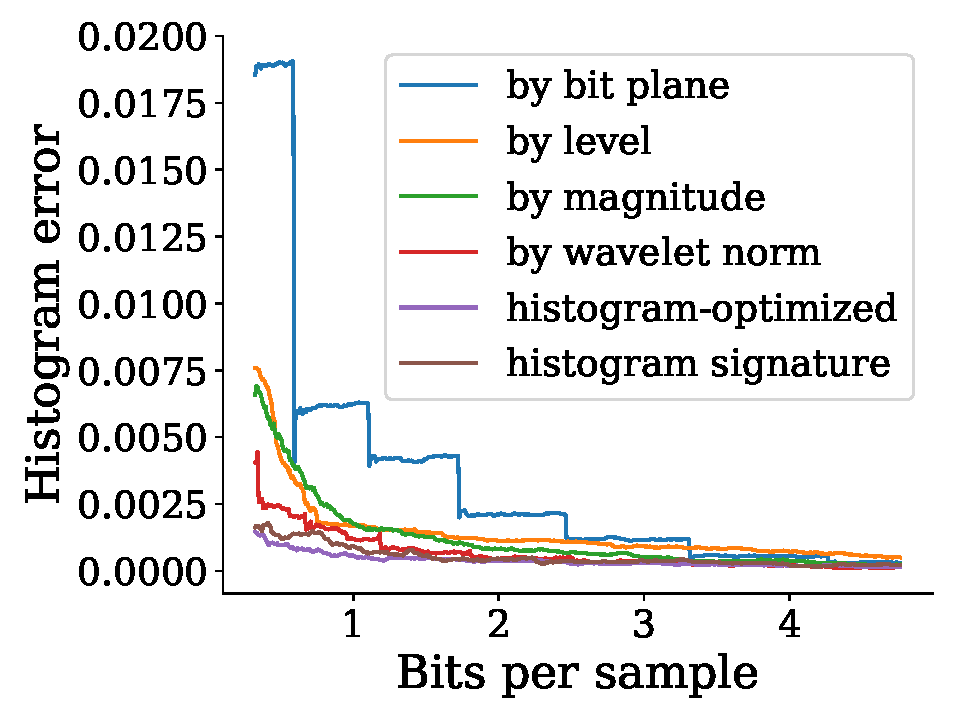
\includegraphics[width=0.24\linewidth]{histogram/histogram-optimized-foam}}
        \caption{Comparison of histogram errors among streams. Plots are truncated to highlight
        differences without hiding important trends. In general, in terms of error, $\shop \approx \shsg
        \approx \swav < \slvl, \sbit, \smag$. The erratic behavior at the beginning for \emph{kingsnake}
        is likely due to the data being too noisy. The especially poor performances of \sbit for
        \emph{boiler} and \emph{foam} are due to the ``shifting'' effect explained in~\Cref{sec:gradient}.
        Crossover points between \sbit and \slvl are explained in~\Cref{fig:histogram-explain}.}
        \label{fig:histogram-stream-comparison}
\vspace{1em}

        \centering
        \subcaptionbox{\emph{by level} (\slvl)}{
        {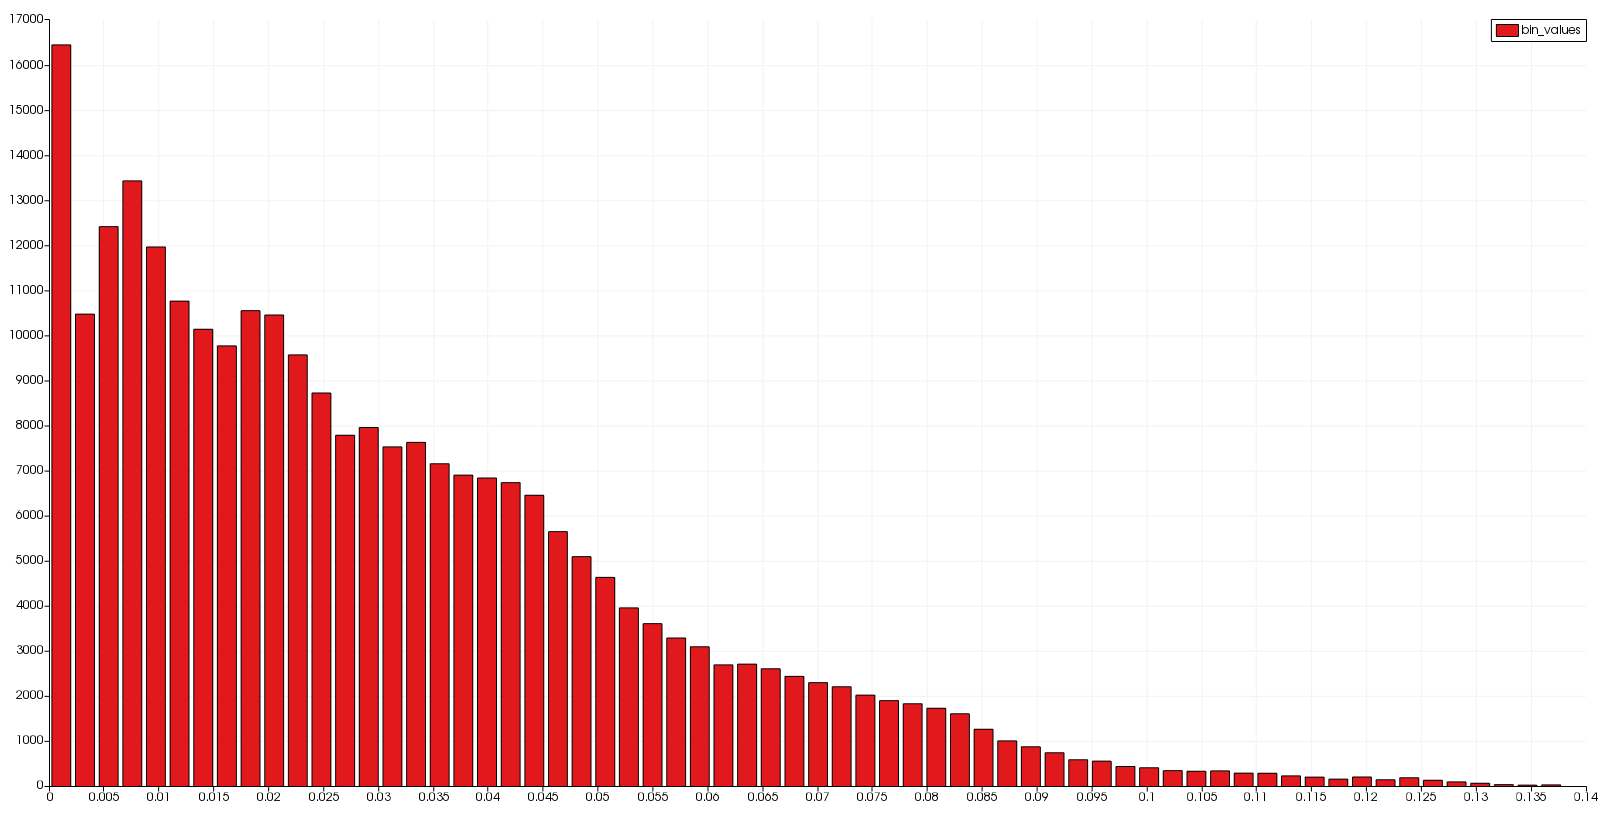
\includegraphics[width=0.158\linewidth]{histogram/histogram-boiler-level}}}
        \subcaptionbox{\emph{by bit plane} (\sbit)}{
        {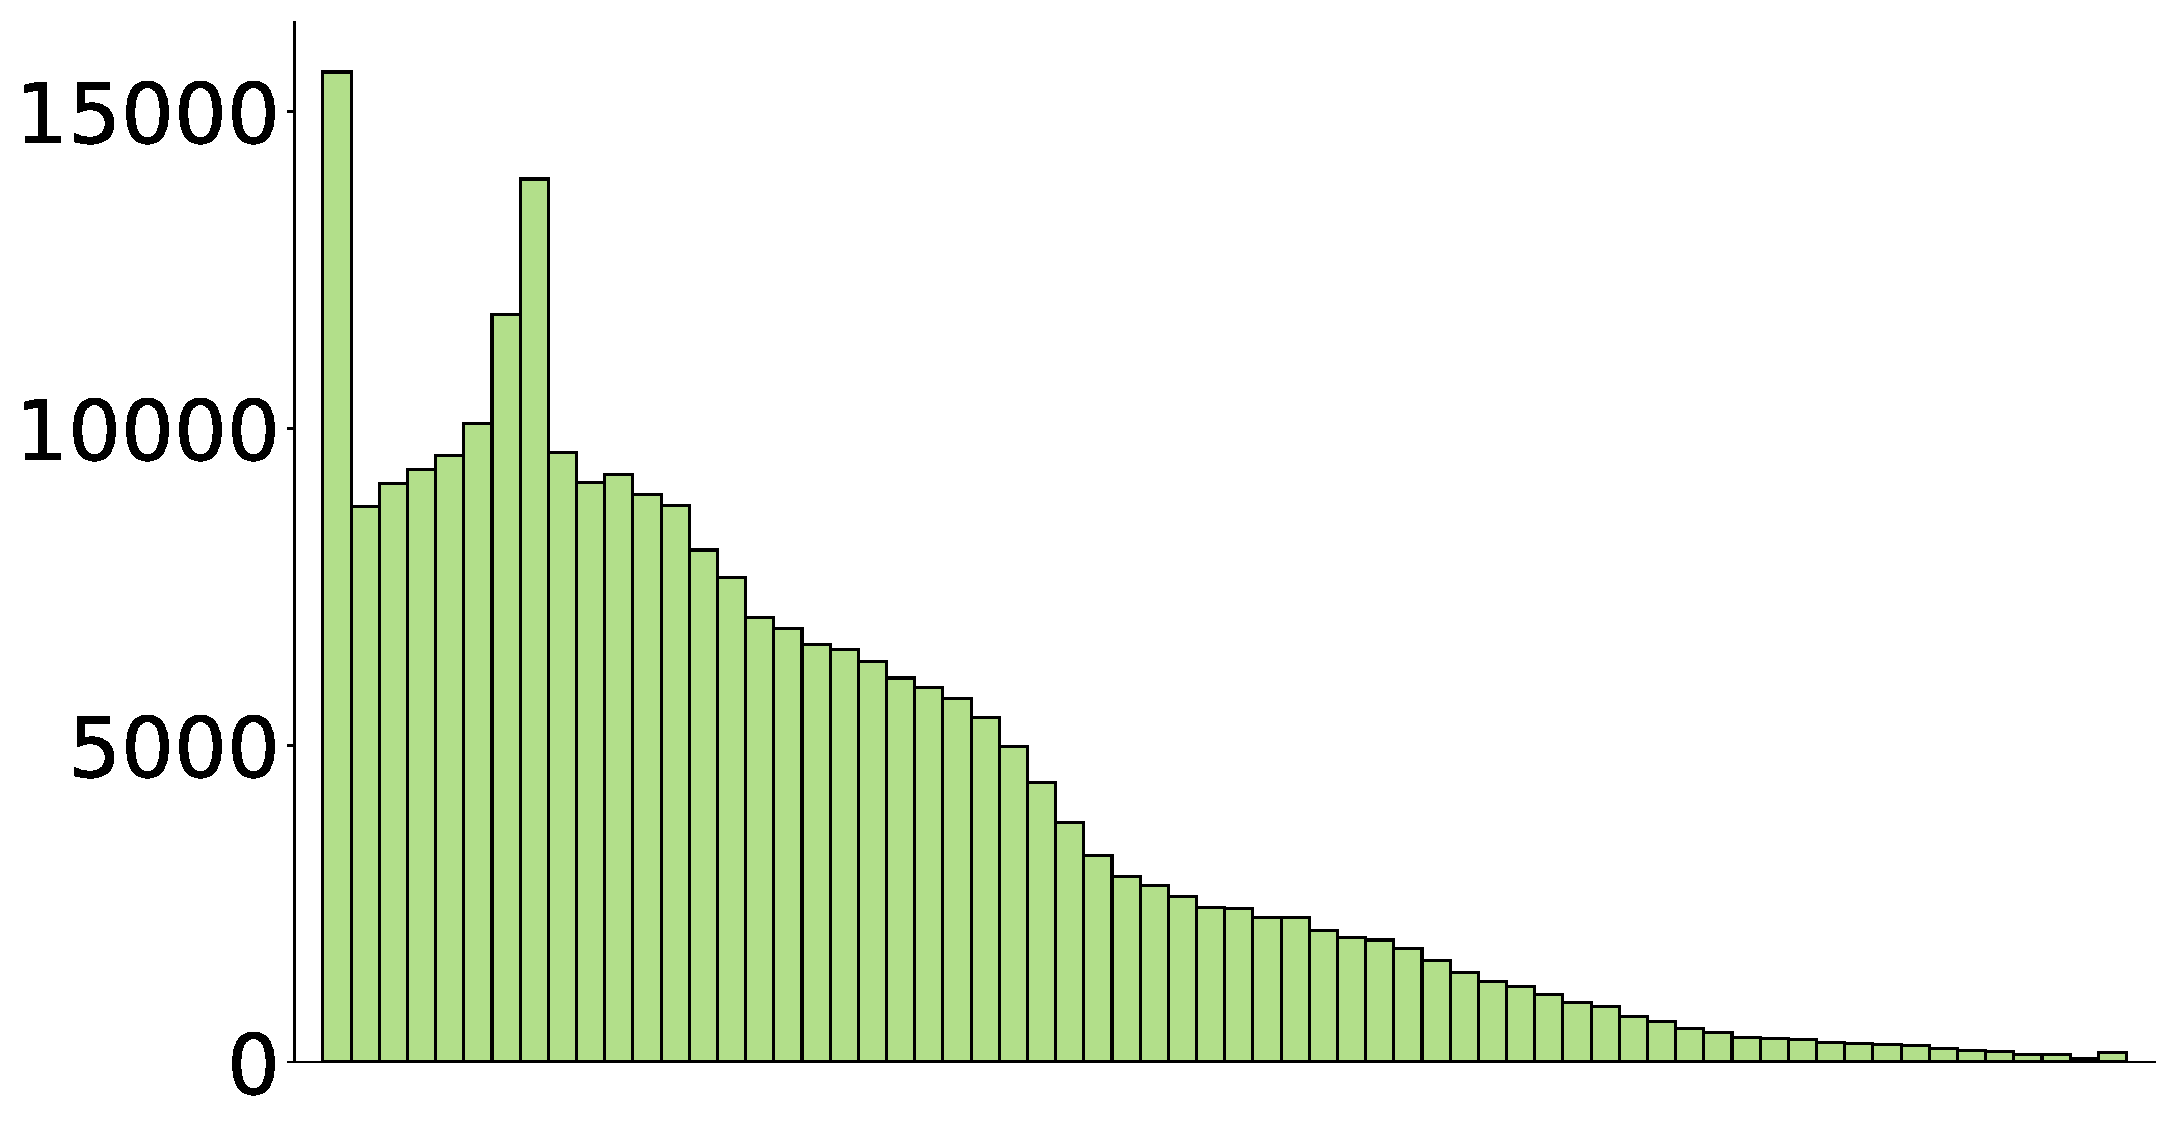
\includegraphics[width=0.158\linewidth]{histogram/histogram-boiler-bit-plane}}}
        \subcaptionbox{\emph{by magnitude} (\smag)}{
        {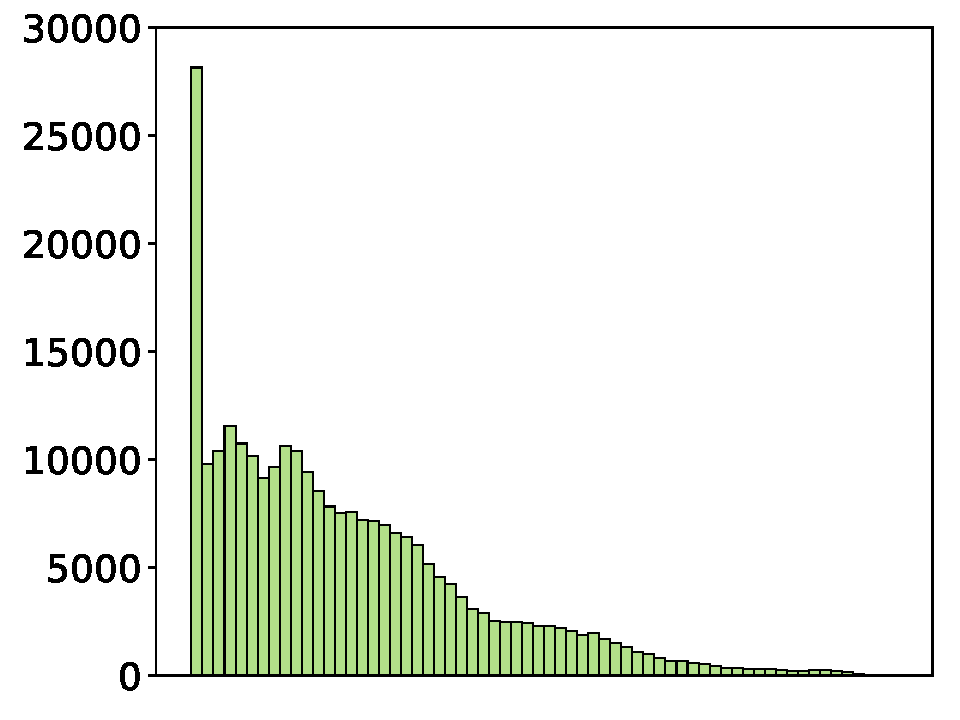
\includegraphics[width=0.158\linewidth]{histogram/histogram-boiler-magnitude}}}
        \subcaptionbox{\emph{by wavelet norm} (\swav)}{
        {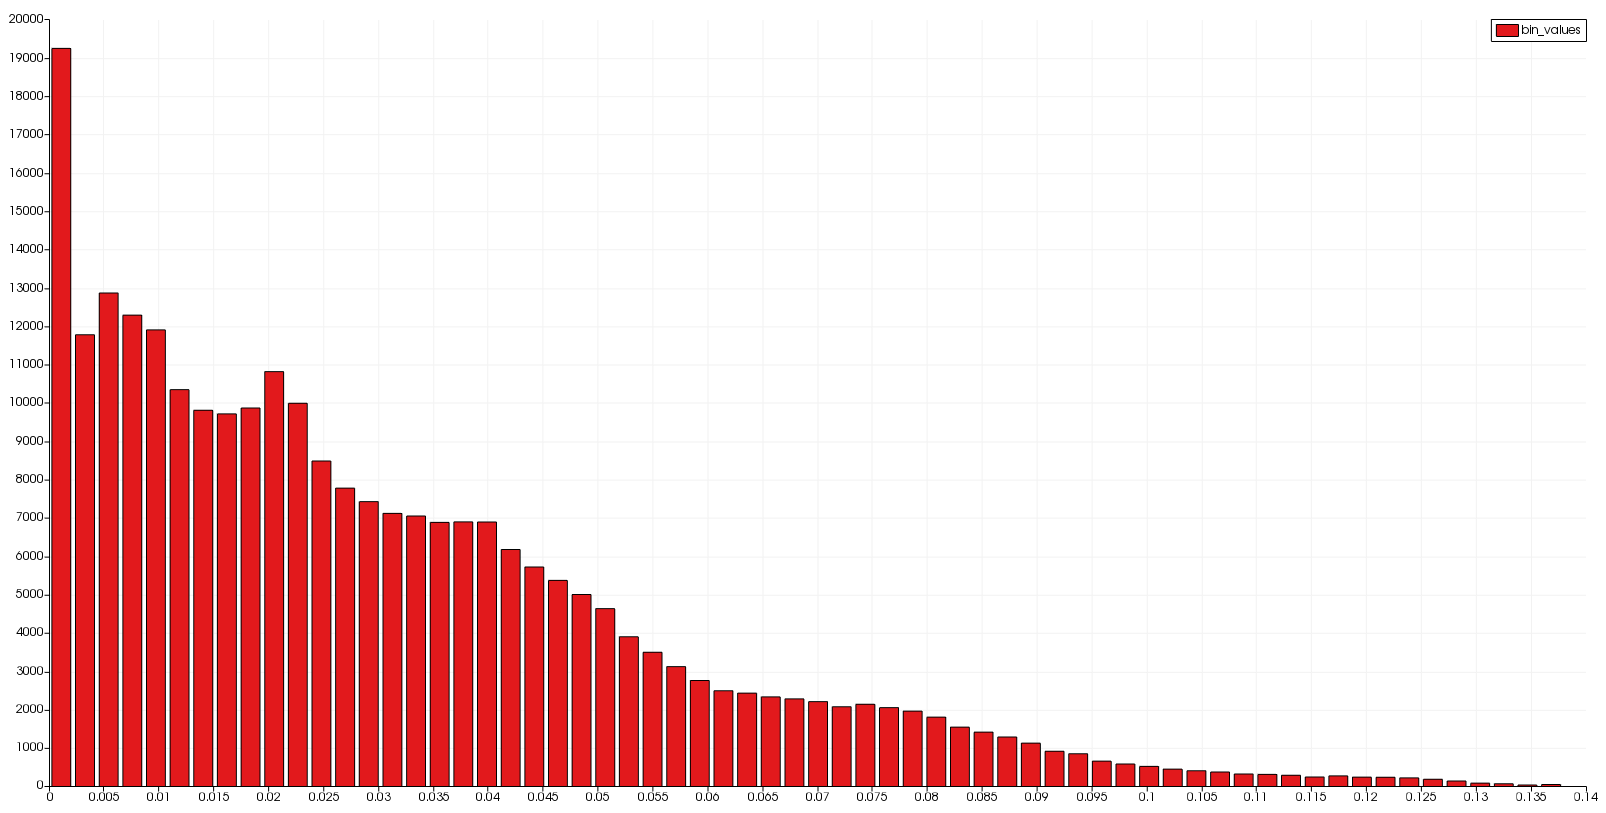
\includegraphics[width=0.158\linewidth]{histogram/histogram-boiler-wavelet-norm}}}
        \subcaptionbox{\emph{by signature} (\shsg)}{
        {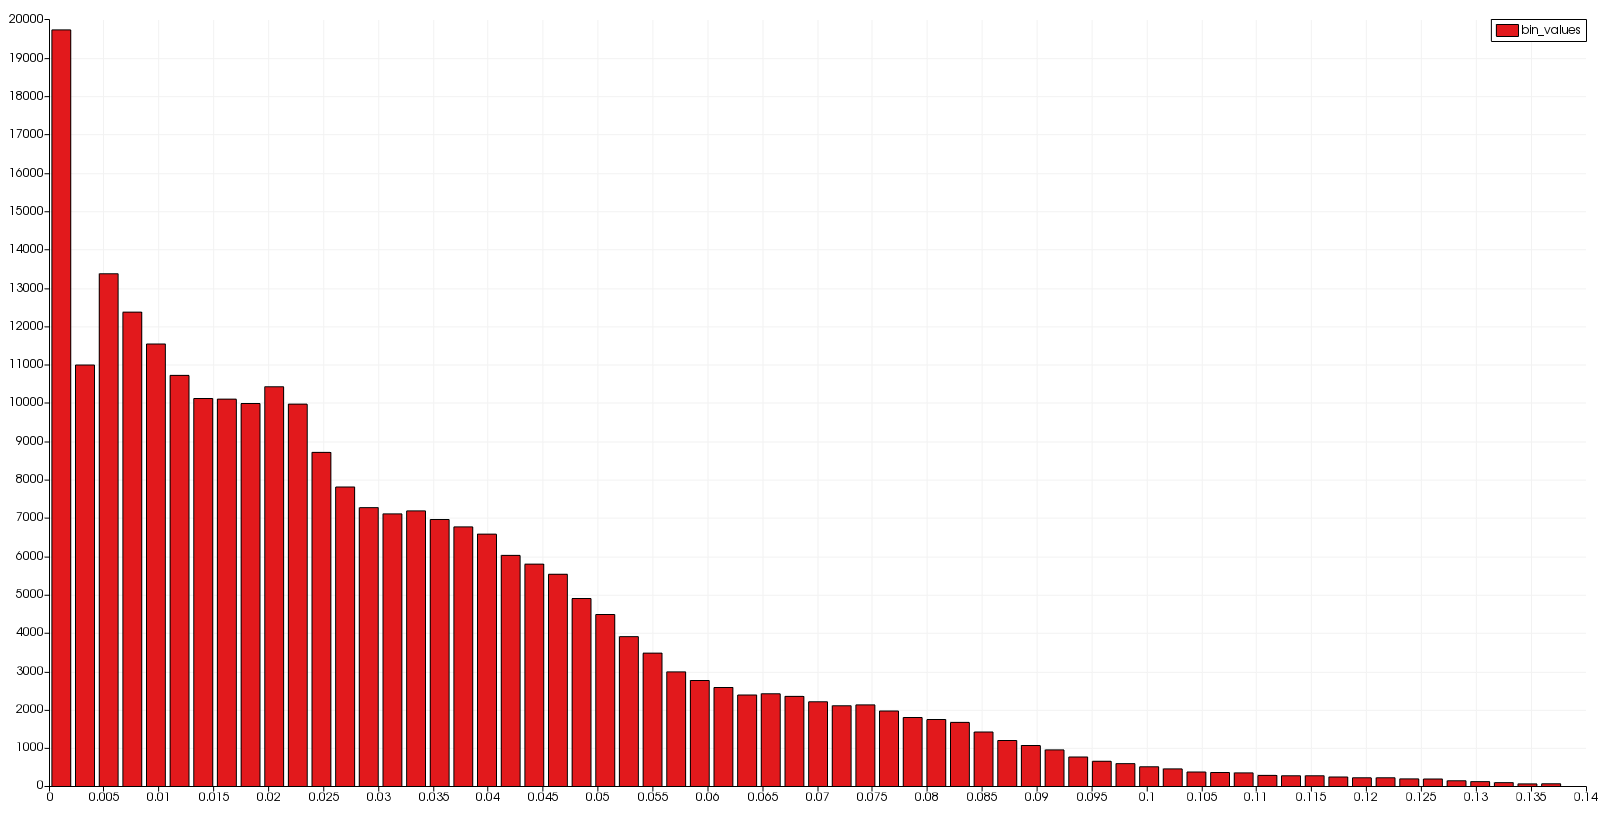
\includegraphics[width=0.158\linewidth]{histogram/histogram-boiler-signature}}}
        \subcaptionbox{\emph{reference}}{
        {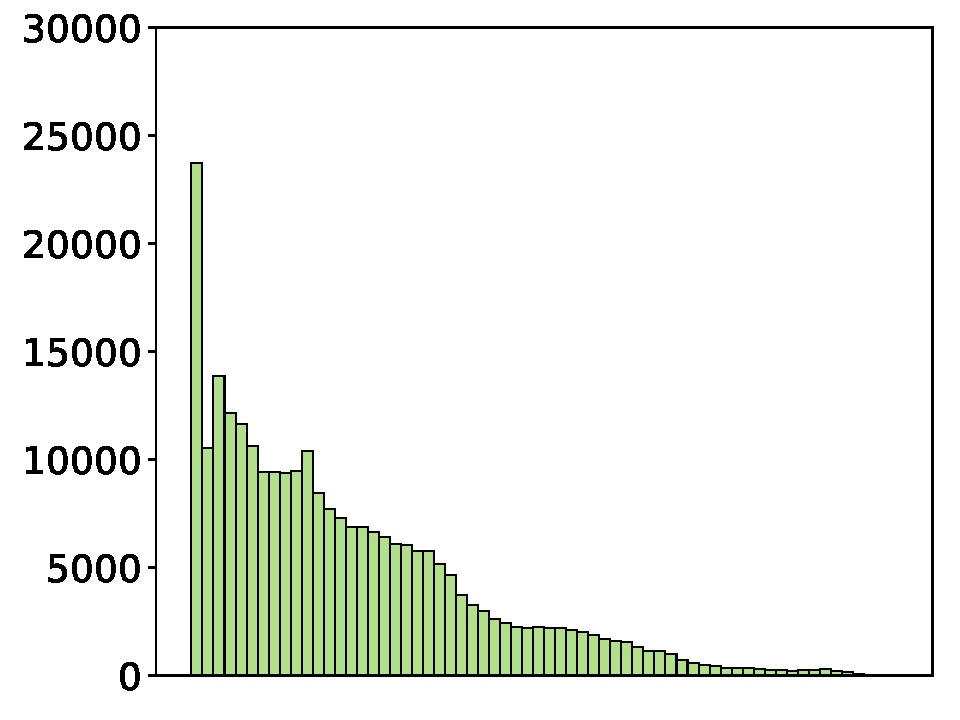
\includegraphics[width=0.158\linewidth]{histogram/histogram-boiler-groundtruth}}}
        \caption{Histograms of the \emph{boiler} data set, reconstructed at 0.3 bps. \slvl, \swav, and
        \shsg produce histograms that share a shape similar to the reference histogram, with most of the
        peaks and valleys preserved. In contrast, \sbit produces a spurious peak not found in the
        reference. Finally, \smag's histogram has a widely skewed distribution where too many values fall
        into the first bin.}
        \label{fig:histograms-boiler}
        \vspace{-1em}
\end{figure*}

\subsubsection{Gradient Computation} \label{sec:gradient}

Given a function $f$ defined on a grid, its gradient at a grid point \mbox{$\x = (x,y,z)$} is the
vector $\nabla f(\x) = \left(\frac{\partial f}{\partial x}, \frac{\partial f}{\partial y},
\frac{\partial f}{\partial z}\right)$. We use a five-point stencil to compute the gradient, i.e.,
$\frac{\partial f}{\partial x} \approx \frac{1}{12}f(x-2,y,z) - \frac{2}{3}f(x-1,y,z) +
\frac{2}{3}f(x+1,y,z) - \frac{1}{12}f(x+2,y,z)$. The error between a gradient field $\nabla f$, and
its low-bit-rate approximation $\nabla
\tilde{f}$, is defined as $\err(\nabla \tilde{f}, \nabla f) = \sqrt{\frac{1}{N}
\sum_{i=1}^{N}{\norm{\nabla \tilde{f}(\x_i)-\nabla f(\x_i)}^2}}$. Using~\Cref{alg:greedy}, we
compute a \emph{gradient-optimized} stream, \sgop, i.e., a stream that minimizes the difference
between the reconstructed gradient field and the original gradient field.

\Cref{fig:gradient-error-comparison} shows the gradient error incurred by different streams for four
data sets. In general, we observe the ordering of performance (from best to worst) as: \sgop, \sgsg,
\sbit, \swav, \smag, \slvl. This ordering can also be seen in~\Cref{fig:gradient-rendering-diff},
where the $x$-component of the gradient field for \emph{tuburlence} is rendered at 0.3 bps. Unlike
the RMSE case, \sbit performs nearly the same as \swav does.

We further investigate this difference by extracting a 1D line from the \emph{plasma} data set and
reconstructing the function using \sbit and \swav at 0.6 bps
(\Cref{fig:bit-plane-vs-wavelet-norm-gradient}).\swav's reconstruction is ``smoother'' and more
accurate \emph{on average}, but lacks the resolution to resolve the high-gradient areas. This is
because \swav intersperses resolution-improving packets and precision-improving packets, unlike
\sbit, which always streams packets that improve resolution first. \sbit, on the other hand, tends
to capture well the function's shape (due to fine-scale bits), but the whole function can be
``shifted'' slightly as seen in the figure, due to the lack of precision in the coarse-scale
coefficients. However, the gradient operator has the tendency to cancel this shifting effect. \sbit,
therefore, might work slightly better than \swav for gradient computation, because it is better able
to retain sharp features.

\begin{figure}[!b]
\centering
\subcaptionbox{\emph{by bit plane}
(\sbit)}{{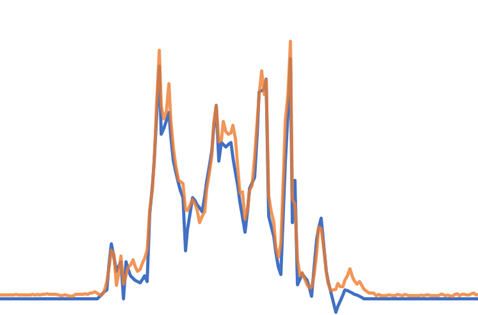
\includegraphics[width=0.48\linewidth]{gradient/1d_plasma_by_bit_plane}}}
\subcaptionbox{\emph{by wavelet norm}
(\swav)}{{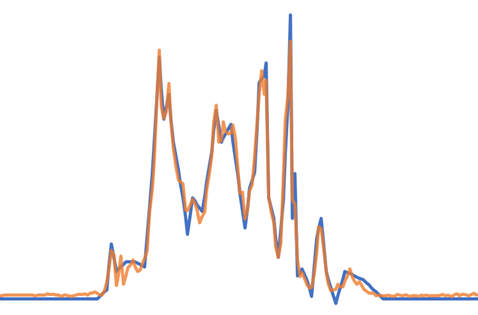
\includegraphics[width=0.48\linewidth]{gradient/1d_plasma_by_wavelet_norm}}} \caption{A 1D
line extracted from \emph{plasma}, and reconstructed using \sbit and \swav at 0.6 bps. The original
data is in orange and the reconstructions are in blue. On average, \swav captures well the function
values, where \sbit struggles (seen as a slight vertical shift). However, \sbit retains the shape of the function slightly better in
high-gradient areas.}
\label{fig:bit-plane-vs-wavelet-norm-gradient}
\vspace{-1em}
\end{figure}

\sgop again outperforms the rest of the streams. \slvl and \smag perform poorly for gradient
computation, lacking the resolution to capture sharp features. \sgsg mostly closely follows \sbit in
performance, but outperforms it for \emph{boiler}. Again, compared to the other fields,
\emph{boiler} is less smooth, resulting in less spatial coherency in the number of leading zero bits
for the fine-scale coefficients, which \sgop and \sgsg can take advantage of, while \swav or \sbit
do not take into account actual bit values. Overall, the results suggest that while \swav is the
best data-independent streams for minimizing RMSE, \sbit is a good alternative for gradient
computation.

\subsubsection{Laplacian Computation}\label{sec:laplacian}

The Laplace operator is a second-order differential operator defined as the divergence of the
gradient field. The Laplacian of a 3D field is defined as $\Delta f = 
\frac{{\partial}^2}{\partial{x^2}}f+\frac{{\partial}^2}{\partial{y^2}}f+\frac{{\partial}^2}{\partial{z^2}}f$.
%
Using a five-point finite difference, we approximate 
%$\frac{{\partial}^2}{\partial{x^2}}f(x,y,z)
$\frac{{\partial}^2 f}{\partial{x^2}}
\approx
-\frac{1}{12}f(x-2,y,z)+\frac{4}{3}f(x-1,y,z)-\frac{5}{2}f(x,y,z)+\frac{4}{3}f(x+1,y,z)-\frac{1}{12}f(x+2,y,z)$.
We use the root-mean-square error to compare two Laplacian fields, i.e., $\err(\Delta
\tilde{f},\Delta f)=\text{RMSE}(\Delta \tilde{f},\Delta f)$. As usual, we use~\Cref{alg:greedy} to
compute a \emph{Laplacian-optimized} stream, \slop, which minimizes $\err$, and an \slsg stream from
its signature.~\Cref{fig:laplacian-error-comparison} plots the error curves for all relevant
streams. The plots here largely follow the ones in~\Cref{fig:gradient-error-comparison}, in terms of
relative performance among the streams, but with more discernible gaps between \sbit and \slsg.



